

\section{Errors}
In this section, we will detail the results that o



%\clearpage
\subsection{Path Jitter}\label{sec:jitter}
The final error that we introduce and simulate is jitter in the path taken by the probe qubits. The precision provided by modern MEMS control structures is about 1 nm \cite{MEMS precision}, 

It was found that adding just a random jitter to the path introduced jumps which the solver could not handle very well. Instead, we overlay a sinusoidal motion over the circular motion, effectively causing a periodic deviation from the perfect path. We introduced a random element in the starting phase and amplitude [check this!] 


\begin{figure}[H]
	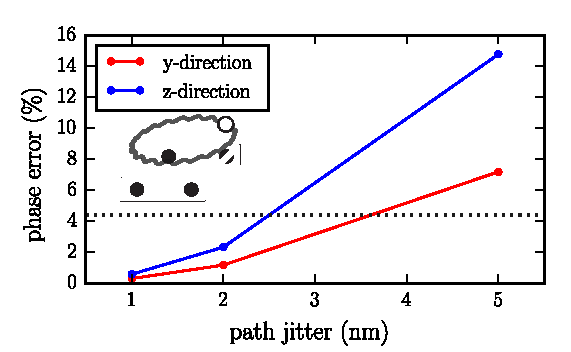
\includegraphics[width=\linewidth]{../Figures/path_jit}
	\caption{}
	\label{FIG:pjit}
\end{figure}


\subsection{Dephasing}
In this section, we present results from simulations of the Lindblad master equation where a dephasing channel is turned on. This channel contains the Lindblad operator
\beq
L  = \sqrt{\Gamma} \sigma_z
\eeq

where $\Gamma$ is the dephasing parameter. $\Gamma$ can also be written as $1/\tau$ where $\tau$ is the dephasing time. We evolve the system under the Lindblad master equation for an odd number of errors. In this simulation, the error is a bit-flip error on the fourth data qubit.  As a result, the probe qubit `backtracks'  during the last quarter of the run such that its final phase ends up at $\phi = \pi$. 

In Figure \ref{fig:BlochsphereDephasing}, we see the effect of a small dephasing coefficient (100) whereas in Figure \ref{fig:BlochsphereDephasing2} we see the effect of larger dephasing (500). Note that the dephasing happens primarily as the interaction between the probe qubit and the data qubit is weak, where the phase of the probe qubit doesn't evolve. 


\begin{figure}[H]
	\subfloat[]{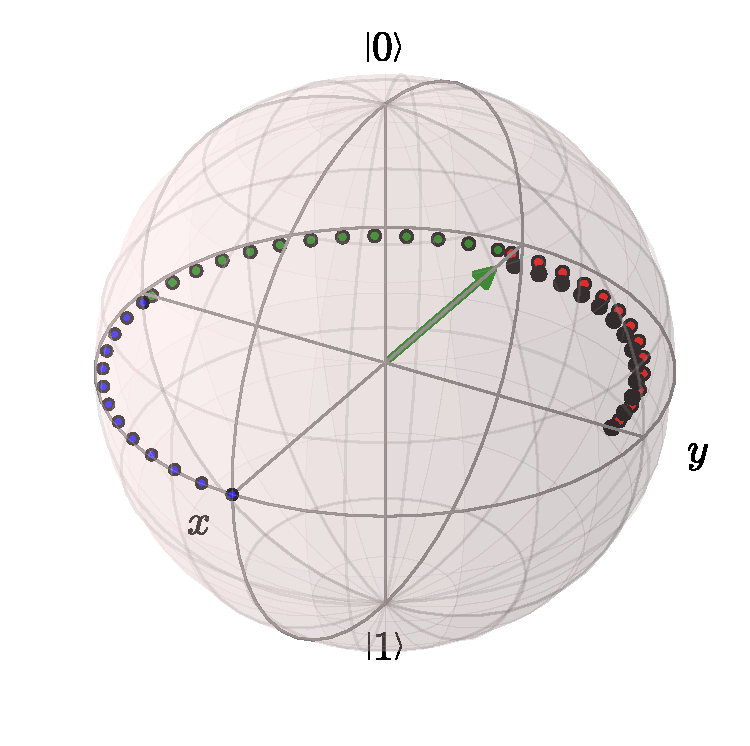
\includegraphics[width=0.49\linewidth]{../Figures/abrupt-deph} \label{FIG:abr-deph}}
	\subfloat[]{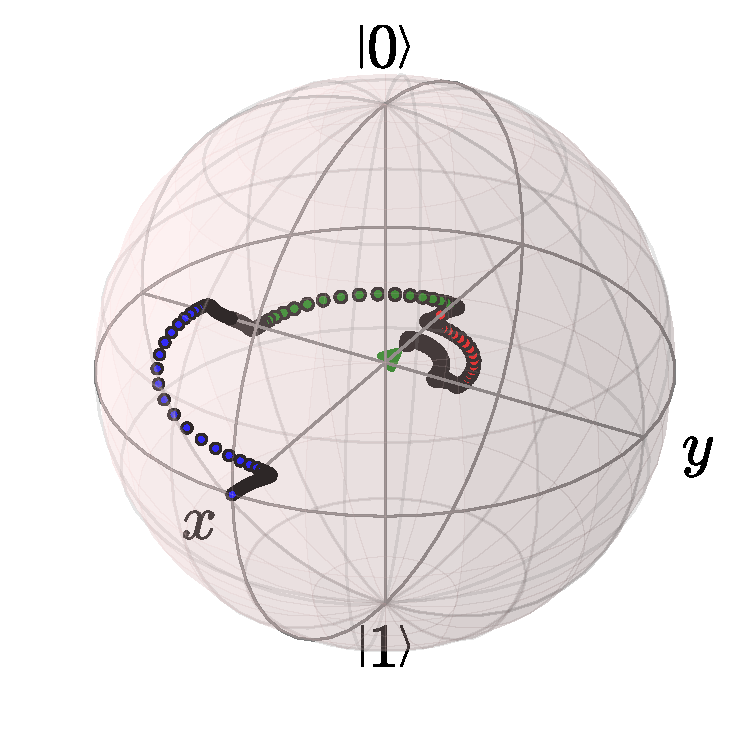
\includegraphics[width=0.49\linewidth]{../Figures/circ-deph} \label{FIG:circ-deph}}
	\caption[oddeven]{}
	\label{FIG:deph}
\end{figure}

\begin{figure}[h]
  \centering
    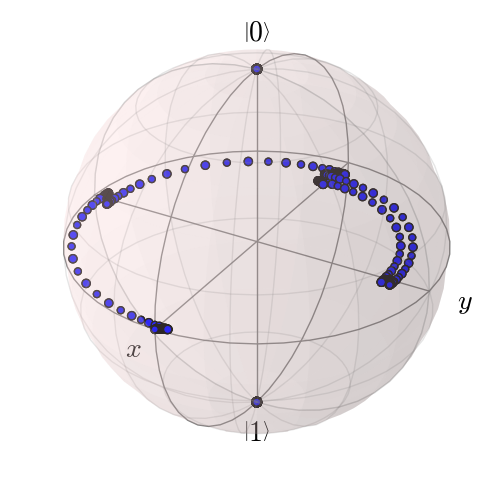
\includegraphics[width=0.5\textwidth]{../Figures/Circ_orbit_odd_100_dephasing.png}
      \caption{The states of the probe and data qubits plotted in the Bloch sphere with a dephasing parameter of 100, which translates to a dephasing time of 10 ms. The phase of the probe qubit is not affected since no relaxation or excitation is taking place. The effect can however be seen in the probability of measuring the probe qubit in the $\ket{+}$ or $\ket{-}$ state. For complete dephasing, the probe qubit will become the maximally mixed state and the measurement outcomes are completely random. The states of the probe and data qubits plotted in the Bloch sphere with a dephasing parameter of 100, which translates to a dephasing time of 10 ms.}
      \label{fig:BlochsphereDephasing}
      
\end{figure}


\begin{figure}[!h]
  \centering
    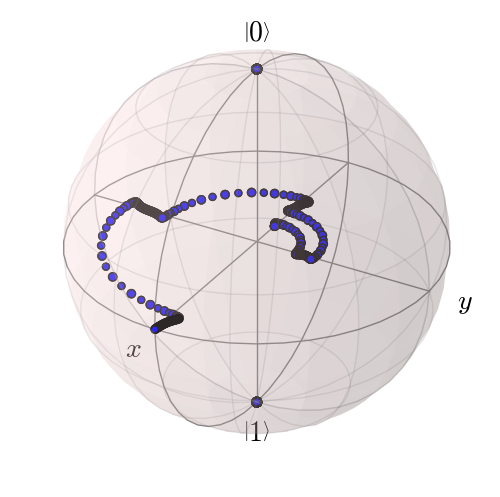
\includegraphics[width=0.5\textwidth]{../Figures/Circ_orbit_odd_500_dephasing.png}
      \caption{The states of the probe and data qubits plotted in the Bloch sphere with a dephasing parameter of 500, which translates to a dephasing time of 2 ms. The strong dephasing causes the probe qubit state to drift quickly towards the maximally mixed state. }
      \label{fig:BlochsphereDephasing2}
\end{figure}

In Figure \ref{fig:phaseplot} we see the effect of dephasing on the probability of measuring the correct value of the probe qubit. Since there is an odd number of errors, we want the probe qubit to end up in the $\ket{-}$ state. However, the dephasing will cause the probe qubit to become a mixed state $\rho$, which means that there is a non-zero probability of measuring $\ket{+} $ instead of $\ket{-}$. For complete dephasing, the probe qubit becomes a mixed state which has a 50--50\% chance of measuring either state. 

\begin{figure}[!ht]
	\centering
	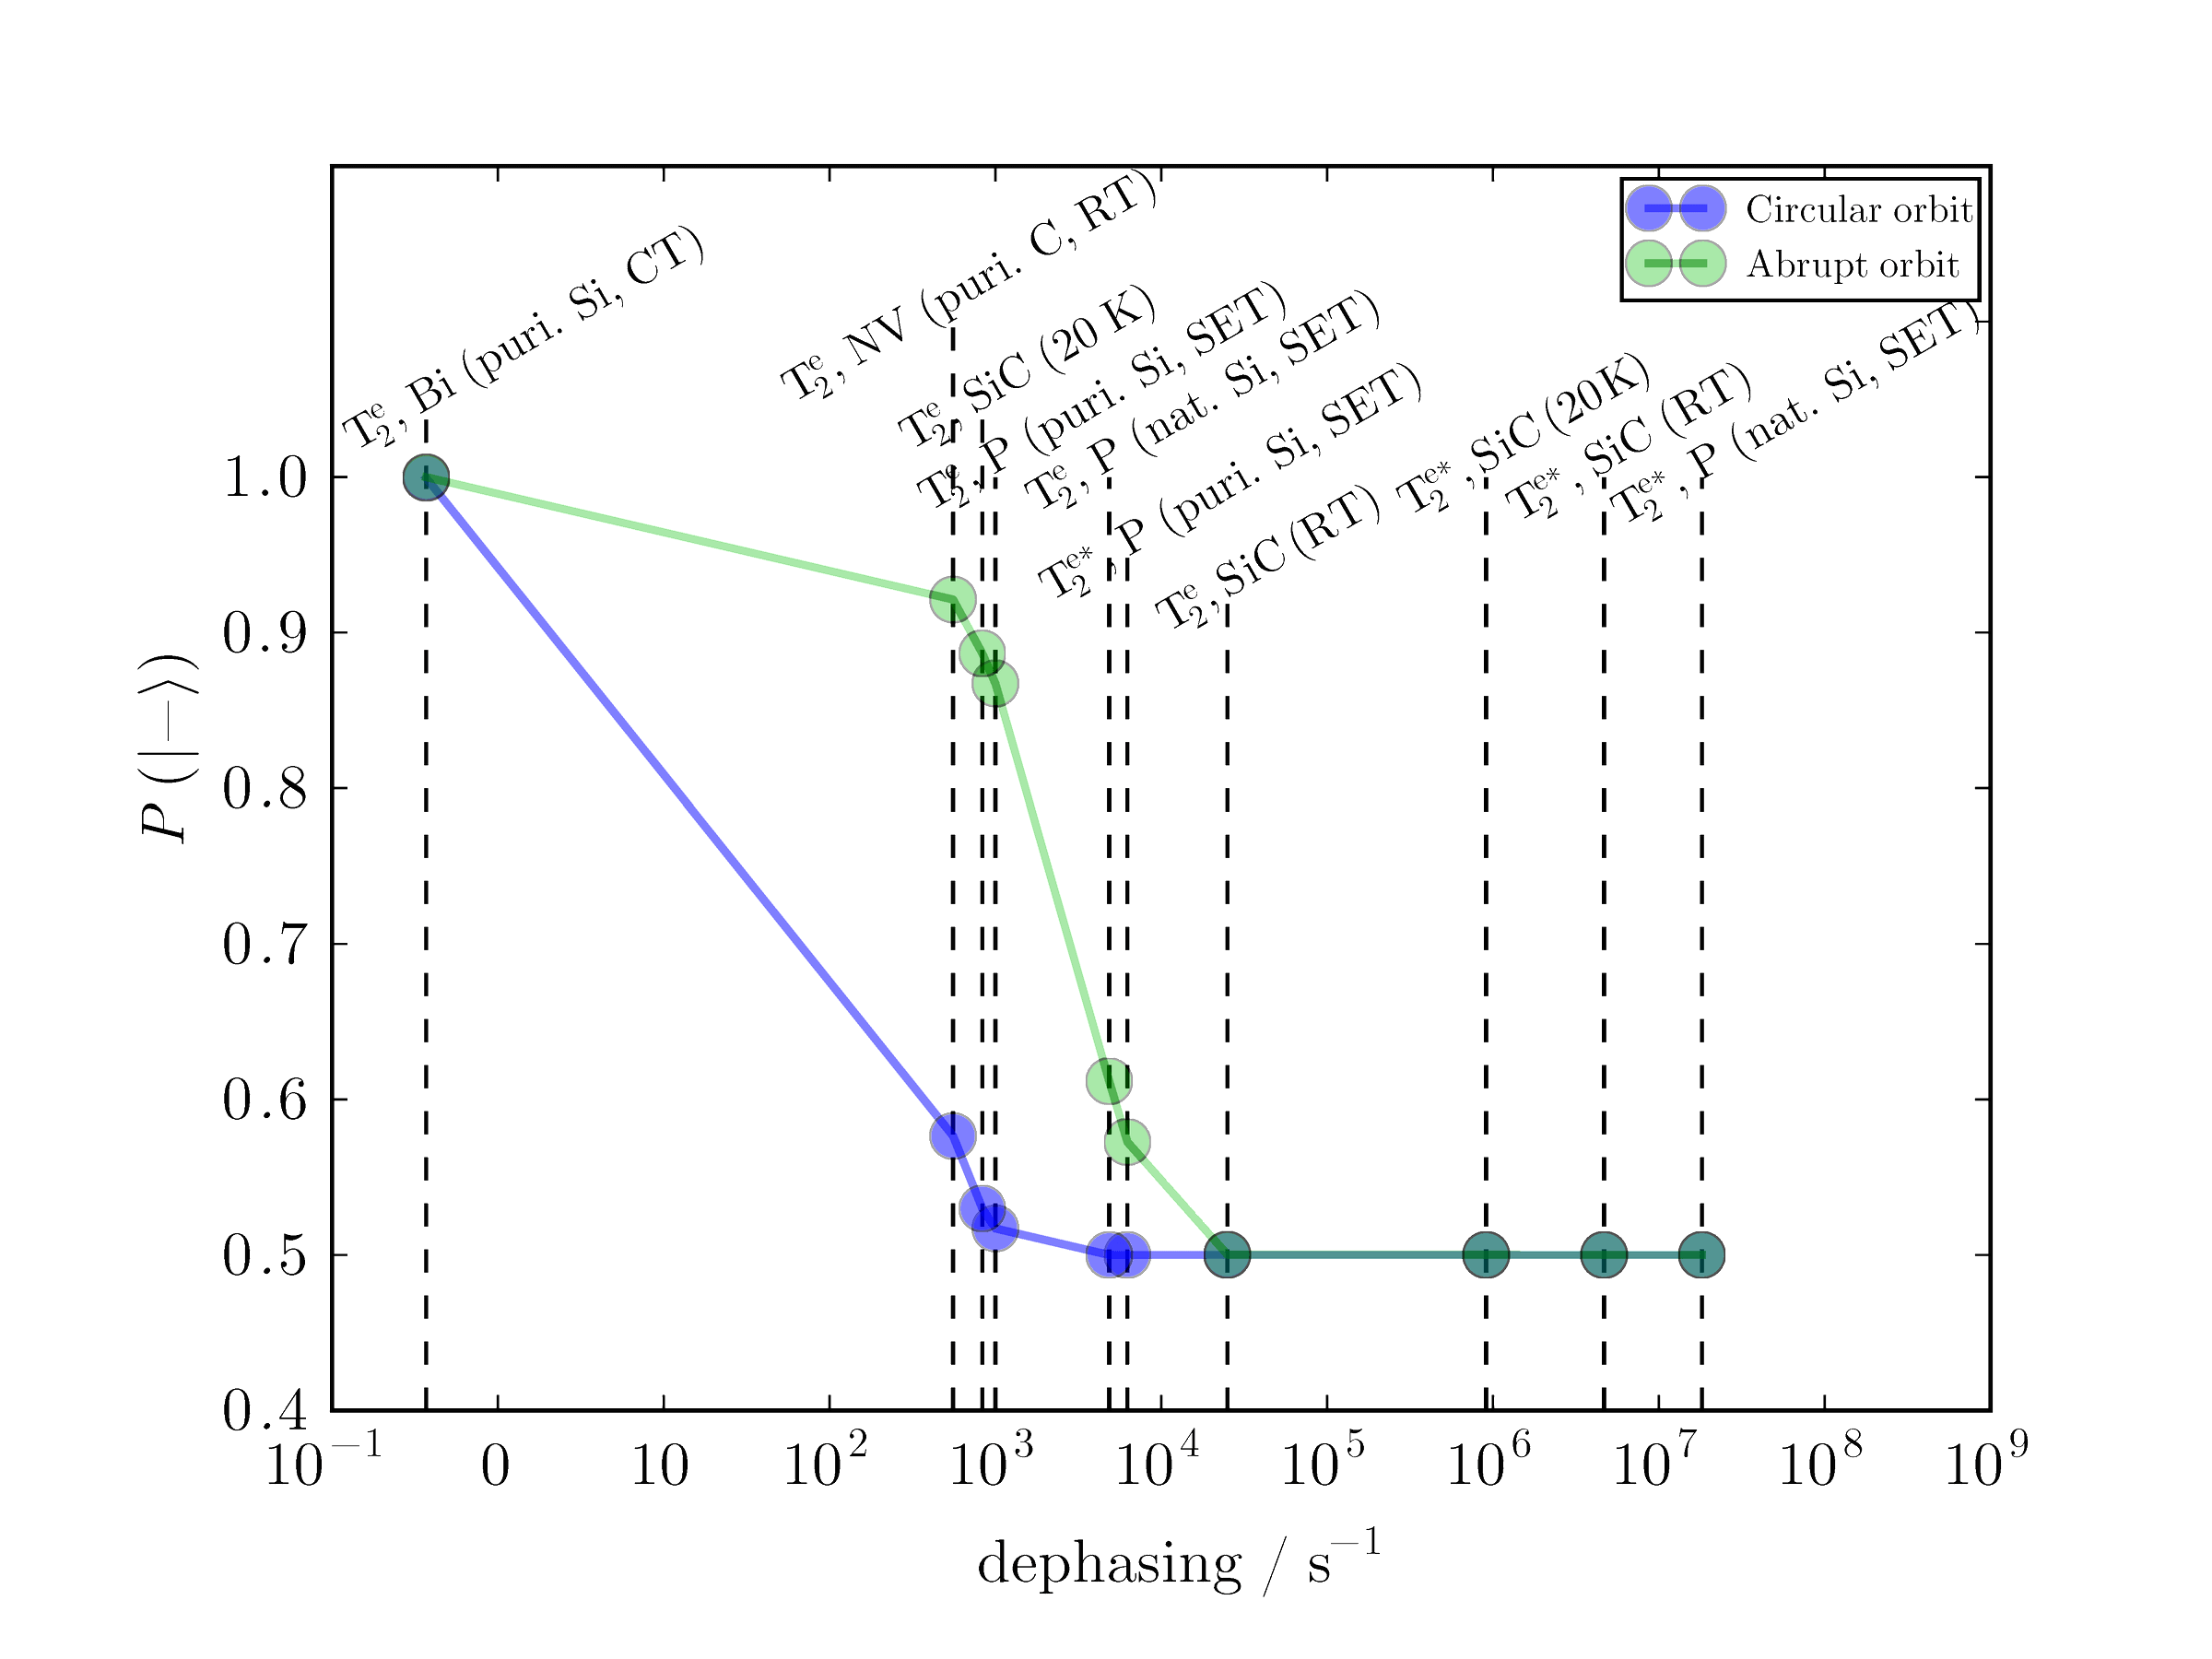
\includegraphics[width=\textwidth]{../Figures/phase_graph.png}
		\caption{A graph showing the relationship between the dephasing parameter $\Gamma$ and the probability $P(\ket{-})$ of measuring the probe qubit in the $\ket{-}$ state. In this simulation, one of the data qubits have undergone a bit-flip error. As the dephasing parameter increases, the probe qubit moves towards the maximally mixed state and the probability of measuring $\ket{-}$ goes towards 0.5. The dephasing parameter for Bismuth as a material for the probe qubit has been market in the graph.}
		\label{fig:phaseplot}
\end{figure}


In Figure \ref{fig:phaseplot}, we have market the data-point for dephasing corresponding to the decoherence time for Bismuth, which is one of the proposed donor types for the probe qubit. The decoherence time of bismuth is \SI{2.7}{\second} \cite{Wolfowicz2013}, which leads to a dephasing parameter of \SI{0.37}{\per\second}. 


It should be noted that the Bismuth dephasing time of 2.7 s can only be obtained by applying advanced Hahn echo readout methods. Whereas it is cumbersome, this technique is not beyond the capabilities of modern experiments. 

